\appendix

\renewcommand{\algorithmicrequire}{\textbf{Input:}}
\newcommand{\deflet}{\textbf{let}}
\newcommand{\mystate}[1]{\STATE \textbf{let} {{}#1}}
\newcommand{\mystop}[1]{\STATE \textbf{stop} \myss{\myangle{{{}#1}}, s'}}
\newcommand{\myss}[1]{${{}#1}$}
\newcommand{\myangle}[1]{\langle {{}#1} \rangle}
\newcommand{\myif}[1]{\IF{\myss{{{}#1}}}}
\newcommand{\myelse}[1]{\ELSIF{\myss{{{}#1}}}}
\newcommand{\SWITCH}[1]{\STATE \textbf{switch} #1\ \textbf{do} \begin{ALC@g}}
\newcommand{\ENDSWITCH}{\end{ALC@g}\STATE \textbf{end switch}}
\newcommand{\CASE}[1]{\STATE \textbf{case} #1\textbf{:} \begin{ALC@g}}
\newcommand{\ENDCASE}{\end{ALC@g}}
\newcommand{\CASELINE}[1]{\STATE \textbf{case} #1\textbf{:} }
\newcommand{\DEFAULT}{\STATE \textbf{default:} \begin{ALC@g}}
\newcommand{\ENDDEFAULT}{\end{ALC@g}}
\newcommand{\DEFAULTLINE}[1]{\STATE \textbf{default:} }




\section{The Security Proofs of UPPRESSO}
\label{ape:model}
In this section, 
we  formally analyze  the security properties of UPPRESSO based on the Dolev-Yao style web model~\cite{SPRESSO}, which has been widely used in the formal analysis of SSO protocols such as OAuth 2.0~\cite{FettKS16} and OIDC~\cite{FettKS17}.
That is, at the first, we give the detailed introduction about how to  indicate the entities (e.g., servers) and communications (e.g., HTTP request) of the web system with Dolev-Yao style web model.
Then, we describe the model of frequent used data format (e.g., HTTP package) and entity  (e.g., browser). 
Following, we present the modelling UPPRESSO system, containing the servers, scripts and the communications among them.
Finally, we give the security proofs of UPPRESSO, that capture the tracks of all essential data, such as identity token, from its birth to being consumed, to guarantee the integrity and confidentiality.
The data tracing is based on the well-built model.    




%For brevity, we focus on the modifications introduced by UPPRESSO in this paper and neglect the proofs for the security of DNS and HTTPS requests. We refer interested readers to~\cite{SPRESSO} for details.

\subsection{The Web Model}
\label{subsec:webmodel}
The Dolev-Yao model abstracts the entities in a system, such as browsers and web servers, as {\em atomic processes}, which communicate with each other through the {\em events}. \cite{SPRESSO} also defines {\em scripting processes} to model client-side scripting such as JavaScript, so a web system consists of a set of atomic and scripting processes. The state of a system, called a {\em configuration}, consists of the current states of all atomic processes and all the events that can be accepted by these processes. We list the definitions of these notations as below~\cite{SPRESSO}.

\vspace{1mm}
\noindent{\em Messages} 
are defined as formal terms without variables (i.e., ground terms) over a {\em signature}. 
The signature $\Sigma$ consists of a finite set of function symbols (with arity). For messages in this mode, the signature $\Sigma$ contains constants such as ASCII strings and nonce, sequence symbols such as n-ary sequences $\langle \rangle$, $\langle . \rangle$, $\langle . ,. \rangle$, and function symbols that model cryptographic primitives such as $\mathtt{encrypt}, \mathtt{decrypt}$ and digital signatures. For example, an HTTP request can be modeled as a ground term containing a type (e.g., $\mathtt{HTTPReq}$), a nonce, a method (e.g., $\mathtt{GET}$ or $\mathtt{POST}$), a domain, a path, URL parameters, request headers and a message body, over the $\Sigma$ in the sequence symbol format. So,
an HTTP GET request for the domain {\sf exa.com/path?para=1} with empty header and body can be represented as: $m:=\langle\mathtt{HTTPReq},n,\mathtt{GET},exa.com,/path,\langle \langle para, 1\rangle \rangle ,\langle \rangle,\langle \rangle \rangle$.

\vspace{1mm}
\noindent{\em Events} are the basic communication elements in the model. An event contains the addresses of sender and receiver, and a message.
An event is of the form $\langle a, f, m \rangle$, where $a$ and $f$ represent the addresses of the sender and receiver respectively, and $m$ is the message to be transmitted.

\vspace{1mm}
\noindent{\em Atomic Processes.} An {\em atomic Dolev-Yao (DY) process} is a tuple $p=$ $(I^p, Z^p, R^p,s_0^p )$, where $I^p$ is the set of addresses that the process listens to, $Z^p$ is the set of states (i.e., a set of terms) that describes the process, $s_0^p$ is an initial state, and $R^p$ is the mapping from an input state $s \in Z^p$ and an event $e$ to a new state $s'$ and an event $e'$. It is worth noting that for one process in a state, only a finite set of events can be accepted by the process as the state and event are defined as the input of $R^p$.
Each atomic process also contains a set of nonces that it may use.

\vspace{1mm}
\noindent{\em Scripting Processes} represent client-side scripts loaded by the browser to provide server-defined functions to the browser. However, a scripting process must rely on an atomic process, such as the browser, and provide the relation $R$ called by this atomic process.

\vspace{1mm}
\noindent{\em Equational theory} is defined as usual in Dolev-Yao models, which uses the symbol $\equiv$ to represent the congruence relation on terms. For example, $dec(enc(m, k), k)$ $\equiv$ $m$, where $k$ is a symmetric key.

\vspace{1mm}
\noindent {\bf Web system.} We can represent the web infrastructure as a web system of form ($\mathcal{W}$, $\mathcal{S}$, $\mathtt{script}$, $E^0$), where $\mathcal{W}$ is the set of atomic processes containing both honest and malicious processes, $\mathcal{S}$ is the set of scripting processes including honest and malicious scripts, $\mathtt{script}$ is the set of concrete script codes related to specific scripting processes in $\mathcal{S}$, and $E^0$ is the set of events acceptable to the processes in $\mathcal{W}$.

\vspace{1mm}
\noindent A {\em configuration} of this web system is a tuple ($S, E, N$), where $S$ is the current states of all processes in $\mathcal{W}$, $E$ is the set of events that the processes accept, and $N$ is a global sequence of nonces that have not been used by the processes yet.


\vspace{1mm}
\noindent A {\em run step} is the system migrating from configurations ($S, E, N$) to ($S', E', N'$) by processing an event $e \in E$.


\subsection{Data Format}
Here we provide the details of the  format of the frequent used \verb+messages+ to construct the web models.

\vspace{1mm}
\noindent\textbf{HTTP Messages}.
An HTTP request message is the term of the form
\begin{multline*}
\ \ \ \ \ \ \ \ \langle \mathtt{HTTPReq}, nonce, method, host, path, \\
parameters, headers, body\rangle \ \ \ \ \ \ \ \
\end{multline*}
An HTTP response message is the term of the form
\begin{equation*}
    \myangle{\mathtt{HTTPResp}, nonce, status, headers, body}
\end{equation*}
The details are defined as follows:
\begin{itemize}
\setlength\itemsep{-2pt}
 \item \myss{\mathtt{HTTPReq}} and \myss{\mathtt{HTTPResp}} denote the types of messages.
 \item \myss{nonce} is a random number that maps the response to the corresponding request.
 \item \myss{method} is one of the HTTP methods, such as \myss{\mathtt{GET}} and \myss{\mathtt{POST}}.
 \item \myss{host} is the constant string domain of visited server.
 \item \myss{path} is the constant string representing the concrete resource of the server.
 \item \myss{parameters} contains the parameters carried by the url as the form \myss{\myangle{\myangle{name, value}, \myangle{name, value}, \dotsc}}, for example, the \myss{parameters} in the url \myss{http://www.example.com?type=confirm}  is \myss{\myangle{\myangle{type, confirm}}}.
 \item \myss{headers} is the header content of each HTTP messages as the form \myss{\myangle{\myangle{name, value}, \myangle{name, value}, \dotsc}}, such as \myss{\langle\myangle{Referer, http://www.example.com},} \myss{\myangle{Cookies, c}\rangle}.
 \item \myss{body} is the body content carried by HTTP \myss{\mathtt{POST}} request or HTTP response in the form \myss{\myangle{\myangle{name, value}, \myangle{name, value}, \dotsc}}.
  \item \myss{status} is the HTTP status code defined by HTTP standard.
\end{itemize}

\vspace{1mm}\noindent\textbf{URL}.
URL is a term \myss{\myangle{\mathtt{URL}, protocol,host,path,parameters}}, where \myss{\mathtt{URL}} is the type, \myss{protocol} is chosen in \myss{\{\mathtt{S}}, \myss{\mathtt{P}\}} as \myss{\mathtt{S}} stands for HTTPS and \myss{\mathtt{P}} stands for HTTP. The \myss{host, path}, and \myss{parameters} are the same as in HTTP messages.

\vspace{1mm}\noindent\textbf{Origin}.
An Origin is a term \myss{\myangle{host, protocol}} that stands for the specific domain used by the HTTP CORS policy, where \myss{host} and \myss{protocol} are the same as in URL.

\vspace{1mm}\noindent\textbf{POSTMESSAGE}.
PostMessage is used in the browser for transmitting messages between scripts from different origins. We define the postMessage as the form \myss{\myangle{\mathtt{POSTMESSAGE}, target, Content, Origin}}, where \myss{\mathtt{POSTMESSAGE}} is the type, \myss{target} is the constant nonce which stands for the receiver, \myss{Content} is the message transmitted and \myss{Origin} restricts the receiver's origin.

\vspace{1mm}\noindent\textbf{XMLHTTPREQUEST}.
XMLHTTPRequest is the HTTP message transmitted  by scripts in the browser. That is, the XMLHTTPRequest is converted from the HTTP message by the browser. The XMLHTTPRequest in the form \myss{\myangle{\mathtt{XMLHTTPREQUEST}, URL, methods, Body, nonce}} can be converted into HTTP request message by the browser, and \myss{\myangle{\mathtt{XMLHTTPREQUEST}, Body, nonce}}  is converted from HTTP response message.

\vspace{1mm}\noindent\textbf{Data Operation}.
The data used in UPPRESSO are defined in the following forms:
\begin{itemize}
\setlength\itemsep{-2pt}
\item \textbf{Standardized Data} is the data in the fixed format, for instance, the HTTP request is the standardized data in the form \myss{\langle\mathtt{HTTPReq}}, \myss{nonce}, \myss{method}, \myss{host}, \myss{path}, \myss{parameters}, \myss{headers}, \myss{body\rangle}.  We assume there is an HTTP request \myss{r :=}  \myss{\langle\mathtt{HTTPReq}},  \myss{n},  \myss{\mathtt{GET}},  \myss{example.com},  \myss{/path},  \myss{\myangle{}},  \myss{\myangle{}},  \myss{\myangle{}\rangle}, here we define the operation on the $r$. That is, the elements in $r$ can be accessed in the form \myss{r.name}, such that \myss{r.method \equiv \mathtt{GET}},  \myss{r.path \equiv /path} and \myss{r.body \equiv \myangle{}}.
\item \textbf{Dictionary Data} is the data in the form \myss{\myangle{\myangle{name, value}, \myangle{name, value}, \dotsc}}, for instance the \myss{body} in HTTP request is dictionary data. We assume there is a \myss{body := \myangle{\myangle{username, alice}, \myangle{password, 123}}}, here we define the operation on the $body$. That is, we can access the elements in \myss{body} in the form \myss{body[name]}, such that \myss{body[username] \equiv alice} and \myss{body[password] \equiv 123}. We can also add the new attributes to the dictionary, for example after we set \myss{body[age] := 18}, the \myss{body} are changed into\myss{ \myangle{\myangle{username, alice}, \myangle{password, 123}, \myangle{age, 18}}}.
\end{itemize}

\vspace{1mm}\noindent\textbf{Patten Matching}.  We define the term with the variable $*$ as the pattern, such as \myss{\myangle{a, b, *}}.
The pattern matches any term which only replaces the $*$ with other terms. For instance,  \myss{\myangle{a, b, *}} matches \myss{\myangle{a, b, c}}.

\subsection{Browser and Scripting Process Model}
In UPPRESSO, we assume that the browsers are honest, therefore, we only need to analyze how the browsers interactive with the scripts.
We first introduce the windows and documents of the browser model.

\vspace{1mm}
\noindent\textbf{Window}. A window \myss{w} is a term of the form \myss{w = \myangle{nonce, documents, opener}}, representing the  the concrete browser window in the system. The \myss{nonce} is the window reference to identify each windows. The \myss{documents} is the set of documents (defined below) including the current document and cached documents (for example, the documents can be viewed via the ``forward" and ``back" buttons in the browser). The \myss{opener} represents the window in which this window is created, for instance, while a user clicks the href in document \myss{d} and it creates a new window \myss{w}, there is \myss{w.opener \equiv d.nonce}.

\vspace{1mm}
\noindent\textbf{Document}. A document \myss{d} is a term of the form
\begin{multline*}
  \ \ \ \langle nonce, location, referrer, script, scriptstate, \\
  scriptinputs, subwindows, active \rangle \ \ \
\end{multline*}
where document is the HTML content in the window.  The \myss{nonce} locates the document. \myss{Location} is the URL where the document is loaded. \myss{Referrer} is same as the Referer header defined in HTTP standard. The \myss{script} is the scripting process downloaded from each servers. \myss{scriptstate} is define by the script, different in each scripts. The \myss{scriptinputs} is the message transmitted into the scripting process. The \myss{subwindows} is the set of \myss{nonce} of document's created windows. \myss{active} represents whether this document is active or not.

A scripting process is the dependent process relying on the browser, which can be considered as a relation \myss{R} mapping a message input and a message output. And finally the browser will conduct the command in the output message. Here we give the description of the form of input and output.
\begin{itemize}
\setlength\itemsep{-2pt}
\item \textbf{Scripting Message Input. } The input is the term in the form
\begin{multline*}
\langle tree, docnonce, scriptstate, stateinputs,cookies,\\
localStorage, sessionStorage, ids, secret \rangle
\end{multline*}
\item \textbf{Scripting Message Output. }The output is the term in the form
\begin{multline*}
\ \ \ \ \ \langle scriptstate, cookies, localStorage, \\
sessionStorage, command \rangle \ \ \ \ \
\end{multline*}
\end{itemize}
The \myss{tree} is the relations of the opened windows and documents, which are visible to this script. \myss{Docnonce} is the document nonce. The  \myss{Scriptstate} is a term of the form defined by each script. \myss{Scriptinputs} is the message transmitted to script. However, the \myss{scriptinputs} is defined as standardized forms, for example, postMessage is one of the forms of \myss{scriptinputs}. \myss{Cookies} is the set of cookies that belong to the document's origin. \myss{LocalStorage} is the storage space for browser and \myss{sessionStorage} is the space for each HTTP sessions.  \myss{Ids} is the set of user IDs while \myss{secret} is the password to corresponding user ID. The \myss{command} is the operation which is to be conducted by the browser. Here we only introduce the form of commands used in UPPRESSO system. We have defined the postMessage and XMLHTTPRequest (for HTTP request) message which are the \myss{commands}. Moreover, a term in the form \myss{\myangle{\mathtt{IFRAME}, URL, WindowNonce}} asks the browser to create this document's subwindow and it visits the server with the URL.



\subsection{Model of UPPRESSO}
In this section, we introduce the model of processes in UPPRESSO system, including IdP server process, RP server process, IdP scripting process and RP scripting process. We will focus on the state form and relation $R$. They can describe that what kind of event can be accepted by the process in each state, and the content of new output events and states.

To be noticed is that, we only focus on the model of servers, browsers and the plain message transmissions among them in this paper, and neglect the HTTPS requests and other necessary Internet facilities (e.g., DNS server) deployed in the UPPRESSO system. 
Because we assume that the internet architecture is well  built and HTTPS is well implemented, so that an adversary cannot conduct the attacks targeting these elements.
\subsubsection{IdP Server Process}
The state of IdP server process is a term in the form \myss{\myangle{ID, SignKey, sessions, users, RPs, Validity, Tokens}}. Other data stored at IdP but not used during SSO authentication are not mentioned here.
\begin{itemize}
\setlength\itemsep{-2pt}
\item \myss{ID} is the identifier of IdP.
%\item \myss{p} is the large prime mentioned before.
\item \myss{SignKey} is the private key used by IdP to generate signatures.
\item \myss{sessions} is the term in the form of \myss{\myangle{\myangle{Cookie, session}}}, the Cookie uniquely identifies the session and sessions store the  browser uploaded messages.
\item \myss{users} is the set of user's information, including  \myss{username, password, ID_U}  and other attributes.
\item \myss{RPs} is the set of RP information which consists of ID of RP \myss{(PID_{RP})}, \myss{Endpoints} (i.e., the set of RP's validity endpoints) and \myss{Validity}.
\item \myss{Validity} is the validity for IdP generated signatures.
\item \myss{Tokens} is the set of IdP generated Identity proofs.
\end{itemize}
To make the description clearer, we also provide the \myss{functions} to define the complicated procedure.
\begin{itemize}
\setlength\itemsep{-2pt}
\item \myss{\mathtt{SecretOfID(u)}} is used to search the user \myss{u}'s password.
\item \myss{\mathtt{UIDOfUser(u)}} is used to search the user \myss{u}'s \myss{ID_U}.
\item \myss{\mathtt{ListOfPID()}} is the set of IDs of registered RP.
\item \myss{\mathtt{EndpointsOfRP(r)}} is the set of endpoints registered by the RP with ID \myss{r}.
%\item \myss{\mathtt{ModPow(a, b, c)}} is the result of \myss{a^b \mod c}.
\item \myss{\mathtt{Multiply(P, a)}} is the result of \myss{aP}, where $P$ is the point on elliptic curve and $a$ is the integer.
\item \myss{\mathtt{CurrentTime()}} is the system current time.
\end{itemize}

The relation of IdP process $R^i$ is shown as Algorithm~\ref{alg1} in Appendix~\ref{ape:alg}.





\subsubsection{RP process}
The state of RP server process is a term in the form \myss{\myangle{ID_{RP}, Endpoints, IdP, Cert, sessions, users}}. Other attributes are not mentioned here.
\begin{itemize}
\setlength\itemsep{-2pt}
\item \myss{ID_{RP}} and \myss{Endpoints} are RP's registered information at IdP.
\item \myss{Cert} is the IdP signed RP information containing \myss{ID_{RP}, Endpoints} and other attributes.
\item \myss{IdP} is the term of the form \myss{\langle ScriptUrl}, \myss{q}, \myss{PubKey \rangle}, where \myss{ScriptUrl} is the site to download IdP script, \myss{q} is the large prime defined before, and \myss{PubKey} is the public key used to verify the IdP signed messages.
\item \myss{sessions} is same as it in IdP process.
\item \myss{users} is the set of users registered at this RP, each user is uniquely identified by the \myss{Account}.
\end{itemize}

The new \myss{functions} are defined as follows:
\begin{itemize}
\setlength\itemsep{-2pt}
 \item \myss{\mathtt{ExEU}(a, q)} is the Extended Euclidean algorithm, which calculates  \myss{a^{-1} \mod q}.
  \item \myss{\mathtt{Random}()} generates a fresh random number.
  \item \myss{\mathtt{RegisterUser}(Account)} add the new user with \myss{Account} into RP's user list.
\end{itemize}
The relation of RP process $R^r$ is shown as Algorithm~\ref{alg2} in Appendix~\ref{ape:alg}.




\subsubsection{IdP scripting process}
The state of IdP scripting process \myss{scriptstate} is a term in the form \myss{\myangle{IdPDomain, Parameters, q, refXHR}}, where
\begin{itemize}
\setlength\itemsep{-2pt}
\item \myss{IdPDomain} is the IdP's host.
\item \myss{Parameters} is used to store the parameters received from other processes.
%\item \myss{p} is the large prime defined before.
\item \myss{q} is used to label the procedure point in the login.
\item \myss{refXHR} is the nonce to map HTTP request and response.
\end{itemize}
The new \myss{functions} are defined as follows.
\begin{itemize}
\setlength\itemsep{-2pt}
 \item \myss{\mathtt{PARENTWINDOW}(tree,docnonce)}. The first parameter is the input relation tree defined before, and the second parameter is the nonce of a document. The output returned by the function is the current window's opener's nonce (null if it doesn't exist nor it is invisible to this document).
  \item \myss{\mathtt{CHOOSEINPUT}(inputs,pattern)}. The first parameter is a set of messages, and the second parameter is a pattern. The result returned by the function is the message in \myss{inputs} matching the \myss{pattern}.
  \item \myss{\mathtt{RandomUrl}()} returns a newly generated host string.
\end{itemize}
The relation of IdP scripting process $script\_idp$ is shown in Appendix~\ref{ape:alg} Algorithm~\ref{alg3}.




\subsubsection{RP scripting process}
The state of RP scripting process \myss{scriptstate} is a term in the form \myss{\langle IdPDomain}, \myss{RPDomain}, \myss{Parameters}, \myss{q}, \myss{refXHR\rangle}. The \myss{RPDomain} is the host string of the corresponding RP server, and other terms are defined in the same way as in IdP scripting process.

Here, we define the function \myss{\mathtt{SUBWINDOW}(tree, docnonce)}, which takes the \myss{tree} defined above and the current document's \myss{nonce} as the input. And it selects the \myss{nonce} of the first window opened by this document as the output. However, if there is no opened windows, it returns  null.

The relation of RP scripting process $script\_rp$ is shown in Appendix~\ref{ape:alg} Algorithm~\ref{alg4}.



\subsection{Proof of Theorem~\ref{the:secure}}


\newtheorem{redef}{Definition}
\newtheorem{req}{Requirement}
\newtheorem{relemma}{Lemma}

We assume that all the network messages are transmitted using HTTPS, postMessage messages are protected by the browser, and the browsers are  honest, so web attackers can never break the security of UPPRESSO.

We provide the detailed proof on the security of UPPRESSO. As analyzed above, the security requirements of UPPRESSO are that the system must ensure only the legitimate user can login an honest RP under her unique account. We consider the visits to RP's resource paths are controlled by the visitors' cookies, so that the attacker can break the security only when he owns the cookie bound to the honest user. Therefore, we can propose the Definition~\ref{def:secure} about the secure UPPRESSO system.
\begin{redef}
Let $\mathcal{UWS}$ be a UPPRESSO web system, $\mathcal{UWS}$ is secure \textbf{iff} for any honest RP $r$ $\in $ $\mathcal{W}$ and  the authenticated cookie $c$ for honest $u$,  $c$ is unknown to the attacker $a$ and only $c$ is used by $u$.
\end{redef}
Therefore, the proof of Theorem~\ref{the:secure} is converted into whether the UPPRESSO system meets the requirement in Definition~\ref{def:secure}. However, as we consider the attacker initially does not know any honest user's cookie, the requirement of Definition~\ref{def:secure} can be separated as the following requirements. Before describing the requirements, we firstly define the user \myss{u}'s authenticated cookie for RP \myss{r} as \myss{c(u,r)}.
\begin{req}
If $c(u,r)$ is the authenticated cookie owned by $u$, $c(u,r)$ cannot be obtained by $a$.
\label{req:cookie1}
\end{req}
\begin{req}
If $c$ is an unauthenticated cookie owned by $a$, $c$ cannot be set as \myss{c(u,r)}.
\label{req:cookie2}
\end{req}
\begin{req}
The user \myss{u} does not use the attacker's cookie (denoted as \myss{c(a,r)}).
\label{req:cookie3}
\end{req}


To prove that UPPRESSO meets the requirements, we now provide the following lemmas. Lemma~\ref{req:cookie1} proves that the UPPRESSO system meets Requirement~\ref{req:cookie1}.
\begin{relemma}
Attacker does not learn users' cookies.
\label{rel:cookie}
\end{relemma}

\begin{proof}
The Brute-force attacks, such as exhausting the possible users' cookies, are infeasible due to the length of cookies. The attackers can only try to obtain the cookies from honest processes in the system.  For an honest user \myss{u} and the honest RP \myss{r}, the valid cookie \myss{c(u,r)} can only be obtained by \myss{u}'s browser \myss{b_u}, the \myss{r}'s script \myss{script\_rp} and RP's server \myss{P^r} .
Here, we only need to prove that the attacker cannot receive the event from these processes which carries \myss{c(u,r)}.
\begin{itemize}
\setlength\itemsep{-2pt}
\item \myss{b.} The browsers are considered honest and well implemented. Therefore, based on the same-origin policy, \myss{b_u} only sends \myss{r}'s cookie to RP's domain, so that attackers cannot receive the cookie.
\item \myss{script\_rp}. According to Algorithm~\ref{alg4}, the \myss{script\_rp} does not send any cookie.
\item \myss{P^r}. According to Algorithm~\ref{alg2}, the \myss{P^r} does not send any cookie.
\end{itemize}
Therefore, Lemma~\ref{rel:cookie} is proved.
\end{proof}

To prove UPPRESSO system meets Requirement~\ref{req:cookie2}, we need to know how the cookie can be set as \myss{c(u, r)}. Based on Algorithm~\ref{alg2}, we propose the following definition.
\begin{redef}
In $\mathcal{UWS}$, the cookie $c$ is to be set as \myss{c(u,r)} only when RP $r$ receives a valid  identity proof (denoted as \myss{t(u,r)} here) of $u$, from the owner of $c$.
\label{red:token}
\end{redef}

To prove that \myss{t(u,r)} cannot be obtained by attackers, we introduce the following lemmas.
\begin{relemma}
Attacker does not learn users' passwords.
\label{rel:password}
\end{relemma}
\begin{proof}
Same as the proof to Lemma~\ref{rel:cookie}, we only need to prove that attackers cannot receive the message from honest processes that carries the password. The honest IdP server is defined as \myss{P^i} and the IdP script is defined as \myss{script\_idp}. Here we give the proof about each processes.
\begin{itemize}
\setlength\itemsep{-2pt}
\item \myss{script\_rp}. According to Algorithm~\ref{alg4}, we can prove that RP script does not send any stored passwords.
\item \myss{P^r}. According to Algorithm~\ref{alg2}, it is easy to find out that RP server does not receive or send any stored passwords.
\item \myss{script\_idp}. Based on Algorithm~\ref{alg3}, we can find that IdP script sends the user's password at Line 68. The target of this message is \myss{Url} whose host is \myss{IdPDoaim} set at Line 67. The \myss{IdPDomian} is set at Line 4 and the value is defined  by the script and never modified. Therefore, the password can only be sent to the IdP server. The IdP server obtains the password at Line 10 in Algorithm~\ref{alg1}  and does not send this parameter to any other processes.
\item \myss{P^i}. Based on Algorithm~\ref{alg1},  we can find that IdP server does not send any stored passwords.
\end{itemize}
Therefore, no attackers can obtain the password from honest processes, so that this lemma is proved.
\end{proof}

\begin{relemma}
Attacker cannot forge or modify the IdP-issued proofs.
\label{rel:signature}
\end{relemma}
\begin{proof}
The IdP-issued proofs include the \myss{Cert} used in \myss{script\_idp}, the \myss{RegistrationResult} and \myss{Token} used in \myss{P^r} . We can easily find that the IdP does not send the private key to any processes so that the attackers cannot obtain the private key. Then we only need to prove that all the proofs are well verified.
\begin{itemize}
\setlength\itemsep{-2pt}
\item \myss{Cert} is used at Line 21, 52 in Algorithm~\ref{alg3}. At Line 21, the \myss{Cert} has already been verified at Line 16. At Line 52, the \myss{Cert} is picked from the state parameters, and the cert parameter is set at Line 19.  At Line 19, the \myss{Cert} has already been verified at Line 16.
At Line 16 the \myss{Cert} is verified with the public key in the scriptstate, where the key is considered initially honest and the key is not modified at Algorithm~\ref{alg3}. Therefore, \myss{Cert} cannot be forged or modified.
\item \myss{RegistrationResult} is used in Algorithm~\ref{alg2} from Line 35 to 55, which is verified at Line 30. The public key is initially set in the RP and never modified. Therefore, \myss{RegistrationResult} cannot be forged or modified.
\item \myss{Token} is used in Algorithm~\ref{alg2} from Line 69 to 84 after Line 65 where it is verified.  As proved before, the public key is honestly set and never modified. Therefore, \myss{Token} cannot be forged or modified.
\end{itemize}
Therefore, this lemma is proved.
\end{proof}

Here we now show the lemma to prove that UPPRESSO meets the requirements in Definition~\ref{red:token} .
\begin{relemma}
Attacker cannot learn users' valid identity proofs.
\end{relemma}
\begin{proof}
As the \myss{Token} has been proved that it can not be forged by the attackers, here we only need to prove that attackers cannot receive \myss{Token} from other honest processes.
\begin{itemize}
\setlength\itemsep{-2pt}
\item Attacker cannot obtain the \myss{Token} from RP server.  We check all the messages sent by the RP server at Line 4, 7, 19, 25, 31, 36, 45, 55, 61, 66, 74, 84 in Algorithm~\ref{alg2}. It is easy to prove that the RP server does not send any \myss{Token} to other processes.
\item Attacker cannot obtain the \myss{Token} from RP script. The  messages sent by RP script can be classified into two classes. 1) The messages at Line 18, 36, 56 in Algorithm~\ref{alg4}  are sent to the RPDomain which is set at Line 4, so that attackers cannot receive these messages. 2) The messages at Line 26,  46 only carry the contents received from RP server, and we have proved that RP server does not send any \myss{Token}. Therefore, attackers cannot receive the \myss{Token} from RP script.
\item Attacker cannot obtain the \myss{Token} from IdP server.  Considering the messages at Line 4, 12, 16, 23, 26, 36, 44, 51, 67 in Algorithm~\ref{alg1}, we find that only the message at Line 67 carries the \myss{Token}. This \myss{Token} is generated at Line 65, following the trace where the \myss{Content} at Line 63, the \myss{PID_U} at Line 61, the \myss{ID_U} at Line 60, the \myss{session} at Line 48, and finally the \myss{cookie} at Line 47. That is, the receiver of \myss{Token}  must be the owner of the \myss{cookie} in which session that saves the parameter \myss{ID_U} . The \myss{ID_U} is set at Line 15 after verifying the password and never modified. As we have already proved that the cookies and passwords cannot be known to attackers,  attackers cannot obtain the \myss{Token} from IdP server.
\item Attacker cannot obtain the \myss{Token} from IdP script. As the proof provided above, only IdP sends the \myss{Token} with the message at Line 67 in Algorithm~\ref{alg1}, the IdP script can only receive the \myss{Token} at  Line 99 in Algorithm~\ref{alg3}. Here we are going to prove that the token \myss{t(u,r)} can only be  sent to the corresponding RP server through IdP script. The receiver of \myss{t(u,r)} is restricted by the \myss{RPOrigin} at Line 100, which is set at Line 55. The host in the \myss{RPOrigin} is verified using the one included in \myss{Cert} at Line 51. If the \myss{Cert} belong to \myss{r}, the attacker cannot obtain the \myss{t(u,r)}. Now we give the proof that the \myss{Cert} belongs to \myss{r}. Firstly we define the negotiated \myss{PID_{RP}} in \myss{t(u,r)} as \myss{p}. That is the \myss{PID_{RP}} at Line 69 in Algorithm~\ref{alg2}  must equal to \myss{p} and the \myss{PID_{RP}} is verified at Line 44 with the \myss{RegistrationToken}. This verification cannot be bypassed due to the state check at Line 60. At the same validity period, the IdP script needs to send the registration request with same \myss{p}  and receive the successful registration result. As the IdP checks the uniqueness of \myss{PID_{RP}} at  Line 32 in Algorithm~\ref{alg1}. The \myss{r} and IdP script must share the same \myss{RegistrationToken}. As the \myss{RegistrationToken} contains the \myss{\mathtt{Hash}(N_U)}, the IdP script and \myss{r} must share the same \myss{ID_{RP}}. Therefore, the  \myss{Cert} saved as the IdP scriptstate parameter must belong to \myss{r}.
\end{itemize}
Therefore, attackers cannot  learn users' valid identity proofs.
\end{proof}
 So far we have proved that UPPRESSO meets the requirements in Definition~\ref{red:token}. Requirement~\ref{req:cookie2} is satisfied.

Then, we prove that UPPRESSO meets Requirement~\ref{req:cookie3}. As the browser follows the same-origin policy,  the attackers cannot set its cookie to user's browser at RP's origin. Therefore, due to Definition~\ref{red:token}, the user only  sets her cookie as \myss{c(a,r)} when RP receives the \myss{Token} containing the attacker's \myss{PID_{U}} and a  valid \myss{PID_{RP}} negotiated by \myss{u} and \myss{r}. It requires that the attackers must know a valid \myss{PID_{RP}}. Here we give a lemma.
\begin{relemma}
Attacker does not know a valid \myss{PID_{RP}} negotiated by user \myss{u} and RP \myss{r}.
\end{relemma}
\begin{proof}
Here we give the proof that attacker cannot obtain the \myss{PID_{RP}} and \myss{N_U} from each processes.
\begin{itemize}
\setlength\itemsep{-2pt}
\item \myss{P^i}. We can find in Algorithm~\ref{alg1}, IdP only returns the message containing \myss{PID_{RP}} to other processes when the \myss{PID_{RP}} is included in the request message.
\item \myss{P^r}. Same as IdP server, RP server only sends the message containing \myss{PID_{RP}}  at Line 55 in Algorithm~\ref{alg2}, and the \myss{PID_{RP}} is contained in the \myss{RegistrationResult} received at Line 28 and verified at Line 44.
\item \myss{script\_rp}. We can find in  Algorithm~\ref{alg4}, RP script  only sends the messages to RP server and IdP script. The receivers' identities are ensured at Line 3, 4. Therefore, attackers cannot obtains the  \myss{PID_{RP}} and \myss{N_U}.
\item \myss{script\_idp}. The HTTP requests sent by IdP script are forwarded to the domain set at Line 4 in Algorithm~\ref{alg3}. The HTTP requests are sent to IdP server. The postMessages are sent to the one set at Line 3, and we will prove the target cannot be attacker.
According to Line 44 in Algorithm~\ref{alg2},  \myss{PID_{RP}} is valid at RP server only when RP server receives the registration result. The \myss{\mathtt{Hash}(N_U)} in the result ensures the result must be issued for the correct \myss{ID_{RP}}. As the registration result is \myss{PID_{RP}}-unique due to Line 32 in Algorithm~\ref{alg1}, the registration result received by IdP script at Line 35 in Algorithm~\ref{alg3} must be same as the one in RP server.
This HTTP response is related with the HTTP request at Line 28, carrying \myss{PID_{RP}} and \myss{\mathtt{Hash}(N_U)} at Line 21, 25. It ensures the \myss{Cert} obtained at Line 15 must belong to RP. As the target at Line 3 is the window which opens the IdP script window and asks for user's login consent, user can easily find out the target site is not coincident with the consent requirement. Therefore, the target cannot be the attacker.
%Here we assume the target is attacker and then the transmitted \myss{PIR_{RP}} and \myss{N_U} cannot be valid at
\end{itemize}
\end{proof}

Therefore, Requirement~\ref{req:cookie3} is satisfied and Theorem~\ref{the:secure} is proved.

\begin{comment}
\subsection{Proof of Theorem~\ref{the:privacy}}
In this section, we give a detailed proof about the privacy of UPPRESSO. That is,  UPPRESSO is a privacy-preserving system, satisfying IdP-Privacy and RP-Privacy. As analyzed above,  the requirements of IdP-Privacy and RP-Privacy are as follows.
\begin{req}
\textbf{IdP-Privacy}. There are honest RPs $r_1, r_2$, IdP $i$ and the honest user $u$. We define the event sets containing each users' login procedure, for instance, the \myss{events_{(u, r_1)}} consists of all the events generated during the \myss{u} logging in to \myss{r_1} in correct procedure. IdP-Privacy requires that for every event $e_1 \in events_{(u, r_1)}$ received by IdP, there is always an  event $e_2 \in events_{(u, r_2)}$, satisfying that $e_1$ and $e_2$ are equivalent.
\label{req:idp}
\end{req}
Here we give the proof that UPPRESSO system meets Requirement~\ref{req:idp}.
\begin{proof}
As IdP is honest, we only need to analyze the events sent to the IdP, to prove the equivalence of these events. The IdP only accepts the HTTPS requests to the path \myss{/script, /synamicRegistration, /login, loginInfo} and \myss{/authorize}, which are examined  as follows.
\begin{itemize}
\item \myss{/script}. Based on Algorithm~\ref{alg1}, we can find that every request to this path does not carry any parameter and body. Therefore, for event $e_1 \in events_{(u, r_1)}$ and $e_2 \in events_{(u, r_2)}$, the HTTPS messages in \myss{e_1} and \myss{e_2} meet the requirements in Definition~\ref{def:httpequ}, so \myss{e_1} and \myss{e_2} are equivalent.
\item \myss{/loginInfo}. As defined in Algorithm~\ref{alg1}, no parameters and bodies are sent to this path. The proof is same as the path \myss{/script}.
\item \myss{/login}. According to Algorithm~\ref{alg1}, the requests carry the body including \myss{u}'s username and password. For event $e_1 \in events_{(u, r_1)}$ and $e_2 \in events_{(u, r_2)}$, the usernames and passwords must be the same. Therefore, \myss{e_1} and \myss{e_2} are equivalent.
\item \myss{/dynamicRegistration}. As defined in Algorithm~\ref{alg1}, the requests should carry the body \myss{PID_{RP}}, \myss{Endpoint} and \myss{Nonce}. That is, the \myss{PID_{RP}} is the result of \myss{ID_{RP}^{N_U} \mod p}, where \myss{N_U} is unknown to IdP. Therefore,  based on Definition~\ref{def:powequ}, the \myss{PID_{RP}} in \myss{e_1} and \myss{e_2} are equivalent. The \myss{Endpoint}s and \myss{Nonce}s are all randomly generated, therefore, they are equivalent in each events. It is proved that \myss{e_1} and \myss{e_2} are equivalent.
\item \myss{/authorize}. Based on Algorithm~\ref{alg1}, it is easy to find that the requests to this path carry the body \myss{PID_{RP}} and \myss{Endpoint} same as in path \myss{/dynamicRegistration}. The proof of equivalence is also same.
\end{itemize}
Therefore, we prove that UPPRESSO meets Requirement~\ref{req:idp}.
\end{proof}

\begin{req}
\textbf{RP-Privacy}. There are RPs $r_1, r_2$, honest IdP $i$ and the honest users $u_1, u_2$. The following requirements are satisfied even if \myss{r_1} and \myss{r_2} share their states.
\begin{itemize}
\item For every event $e_1 \in events_{(u_1, r_2)}$ received by RP, there is always an  event $e_2 \in events_{(u_2, r_2)}$, and $e_1$ and $e_2$ are equivalent.
\item For any user \myss{u}, the event \myss{e \in events_{(u, r_2)}} cannot be linked with a $u$'s \myss{Account} at $r_1$.
\end{itemize}
\label{req:rp}
\end{req}
Here we give the proof that UPPRESSO system meets Requirement~\ref{req:rp}.
\begin{proof}
We first prove that RP-Privacy is satisfied when RPs are honest, and then extend the proof when the RPs behave malicious to use illegal parameters and conduct illegal processes.

%As the RPs are considered malicious, at the beginning of the proof we only focus on the procedure with legal parameters. Then the RPs are considered able to use illegal parameters and conduct illegal processes.

The events known to the RPs include the postMessages sent by IdP script to RP script, and the HTTPS messages sent by RP script to RP server. However, we can find in Algorithm~\ref{alg2} that all the postMessages received by RP script are transmitted to RP server, so that we  only need to analyze the RP's paths for HTTPS requests. For honest RP, the proof is as follows.
\begin{itemize}
\item \myss{/script}. As defined in Algorithm~\ref{alg2}, every request to this path does not carry any parameters and bodies. The HTTPS messages in event $e_1 \in events_{(u_1, r_2)}$ and $e_2 \in events_{(u_2, r_2)}$ are equivalent based on Definition~\ref{def:httpequ}, so \myss{e_1} and \myss{e_2} are equivalent.
\item \myss{/login}. According to Algorithm~\ref{alg2}, the requests to this path do not carry any parameters and bodies. Therefore, same as in path \myss{/script}, \myss{e_1} and \myss{e_2} are equivalent.
\item \myss{/startNegotiation}. Based on  Algorithm~\ref{alg2}, we can find that the requests to this path only carry the body  \myss{N_U}. As \myss{N_U} is a random  number, the messages in \myss{e_1} and \myss{e_2} are equivalent, so \myss{e_1} and \myss{e_2} are equivalent.
\item \myss{/registrationResult}. According to Algorithm~\ref{alg2}, the requests to this path contain the \myss{RegistrationResult} in the body. The \myss{RegistrationResult} includes \myss{PID_{RP}}, \myss{Endpoint}, \myss{Nonce} and the \myss{Validity}. However, the \myss{PID_{RP}} is also a random number (due to the randomness of \myss{N_U}), and \myss{Nonce} is the hash of \myss{N_U}, so \myss{PID_{RP}}s and \myss{Nonce}s are equivalent. \myss{Endpoint} is a  random string. \myss{Validity} is generated based on the current time. Therefore, all the parameters in \myss{e_1} and \myss{e_2} are considered equivalent, so \myss{e_1} and \myss{e_2} are equivalent.
\item \myss{/uploadToken}.  As  defined in  Algorithm~\ref{alg2}, the requests to this path carry the \myss{Token}. \myss{Token} consists of \myss{PID_{RP}}, \myss{PID_U} and \myss{Validity}. As analyzed above, \myss{PID_{RP}}s and \myss{Validity}s in each events are equivalent. \myss{PID_U} is the result of \myss{ID_{RP}^{ID_U} \mod p}, so \myss{PID_U}s are equivalent to RP who doesn't know \myss{ID_U} due to Definition~\ref{def:powequ}. Therefore,  \myss{e_1} and \myss{e_2} are equivalent.
\end{itemize}
Moreover, with the states shared by \myss{r_2}, \myss{r_1} knows  all  the \myss{Account}s at \myss{r_2}. However, as \myss{ID_{RP}}s of \myss{r_1} and \myss{r_2} satisfy the equation \myss{ID_{RP_{r_1}}} \myss{\equiv}  \myss{ID_{RP_{r_2}}^x \mod p} where \myss{x} is unknown to RPs due to the discrete logarithm problem,  the \myss{Account} at \myss{r_2} cannot be linked with the \myss{Account} at \myss{r_1}.

Therefore, the UPPRESSO meets Requirement~\ref{req:rp} when RPs behave honestly.

Here, we prove that UPPRESSO meets the RP-Privacy requirements even when RPs behave maliciously.
The malicious RPs may attempt to steal the data from other process, or set the illegal parameters during the login procedures. That is, according to Definition~\ref{def:powequ}, the $PID_U$s and the $Account$s must be equivalent to the attacker as long as the attacker does not know the $ID_U$. Based on Algorithm~\ref{alg1}, we  find  that IdP does not send \myss{ID_U} to any process, so  $PID_U$s the $Account$s must be equivalent in each event.

Malicious RPs may attempt to generate  \myss{Account} and \myss{PID_U} incorrectly, however, the correct user could find this illegal behaviours as follows.
\begin{itemize}
\item RP may attempt to use a forged $ID_{RP}$ or $PID_{RP}$ to make $PID_U$s or $Accounts$ inequivalent. However, $ID_{RP}$ are provided by the $Cert$, which is verified at Line 17 in Algorithm~\ref{alg3} using the IdP's public key that is initialized correctly and never modified.  $PID_{RP}$ is generated by the $ID_{RP}$ at Line 21 using a nonce generated by the honest user at Line 20. Therefore, the honest user will find the illegal $ID_{RP}$ and $PID_{RP}$.
\item RP may attempt to make the same user  upload the identity proof with same $PID_U$ or $Account$ to break RP-Privacy. However, $PID_U$ is generated with the nonce $N_U$ provided by the user, and will never be controlled by the (malicious) RP. $Account$ is generated using the equation $ID_{RP}^{ID_U} \mod p$, while RPs may lead the user to use the same $ID_{RP}$ to generate identity proof. However, the $ID_{RP}$ is bound with $Cert$ which is verified by the user and it is easy for user to find the incorrect $ID_{RP}$.
\end{itemize}

Therefore,  UPPRESSO system meets Requirement~\ref{req:rp}.
\end{proof}
Finally, we have proved that the UPPRESSO system meets Requirement~\ref{req:idp} and ~\ref{req:rp}, and therefore Theorem~\ref{the:privacy} is proved.
\end{comment}

\onecolumn

\section{Algorithm}
\label{ape:alg}

\subsection{IdP process}
\begin{breakablealgorithm}
  \caption{$R^i$}
  \label{alg1}
  \begin{algorithmic}[1]
  \REQUIRE \myss{\myangle{a, f, m}, s}
  \mystate{\myss{s:=s'}}
  \mystate{\myss{n, method, path, parameters, headers, body} \textbf{such that}}\\
  \ \ \myss{\myangle{\mathtt{HTTPReq},n,method,path,parameters,headers,body} \equiv m}\\
  \ \ \textbf{if} \myss{possible}; \textbf{otherwise} stop \myss{\myangle{}, s'}
  \myif{path \equiv /script}
  \mystate{\myss{m':=\myangle{\mathtt{HTTPResp},n,200, \myangle{}, \mathtt{IdPScript}}}}
  \mystop{f, a, m'}
  \myelse{path \equiv /login}
  \mystate{\myss{cookie := headers[Cookie]}}
  \mystate{\myss{session := s'.sessions[cookie]}}
  \mystate{\myss{username:=body[username]}}
  \mystate{\myss{password:=body[password]}}
  \myif{password \not\equiv \mathtt{SecretOfID}(username)}
  \mystate{\myss{m' :=\myangle{\mathtt{HTTPResp},n,200,\myangle{},\mathtt{LoginFailure}}}}
  \mystop{f,a,m'}
  \ENDIF
  \mystate{\myss{session[uid] := \mathtt{UIDOfUser}(username)}}
  \mystate{\myss{m' :=\myangle{\mathtt{HTTPResp},n,200,\myangle{},\mathtt{LoginSucess}}}}
  \mystop{f,a,m'}
  \myelse{path \equiv /loginInfo}
  \mystate{\myss{cookie := headers[Cookie]}}
  \mystate{\myss{session := s'.sessions[cookie]}}
  \mystate{\myss{username := session[username]}}
  \myif{username \not\equiv \mathtt{null}}
  \mystate{\myss{m' := \myangle{\mathtt{HTTPResp},n,200,\myangle{},\mathtt{Logged}}}}
  \mystop{f,a,m'}
  \ENDIF
  \mystate{\myss{m' := \myangle{\mathtt{HTTPResp},n,200,\myangle{},\mathtt{Unlogged}}}}
  \mystop{f,a,m'}
  \myelse{path \equiv /dynamicRegistration}
  \mystate{\myss{PID_{RP} := body[PID_{RP}]}}
 \mystate{\myss{Endpoint := body[Endpoint]}}
  \mystate{\myss{Nonce := body[Nonce]}}
  \myif{PID_{RP} \in \mathtt{ListOfPID()}}
  \mystate{\myss{Content :=\myangle{Fail, PID_{RP}, Nonce}}}
  \mystate{\myss{Sig := \mathtt{Sig}(Content, s'.SignKey)}}
  \mystate{\myss{RegistrationResult := \myangle{Content, Sig}}}
  \mystate{\myss{m' := \myangle{\mathtt{HTTPResp}, n, 200, \myangle{}, RegistrationResult}}}
  \mystop{f,a,m'}
  \ENDIF
  \mystate{\myss{Validity := \mathtt{CurrentTime} ()+ s'.Validity}}
 \mystate{\myss{s'.RPs := s'.RPs +  ^{\myangle{}} \myangle{PID_{RP}, Endpoint, Validity}}}
  \mystate{\myss{Content := \myangle{OK, PID_{RP}, Nonce, Validity}}}
  \mystate{\myss{Sig := \mathtt{Sig}(Content, s'.SignKey)}}
  \mystate{\myss{RegistrationResult := \myangle{Content, Sig}}}
  \mystate{\myss{m' := \myangle{\mathtt{HTTPResp}, n, 200, \myangle{}, RegistrationResult}}}
  \mystop{f,a,m'}
  \myelse{path \equiv /authorize}
  \mystate{\myss{cookie := headers[Cookie]}}
  \mystate{\myss{session := s'.sessions[cookie]}}
  \mystate{\myss{username := session[username]}}
  \myif{username \equiv \mathtt{null}}
  \mystate{\myss{m' := \myangle{\mathtt{HTTPResp}, n, 200, \myangle{}, \mathtt{Fail}}}}
  \mystop{f,a,m'}
  \ENDIF
  \mystate{\myss{PID_{RP} := parameters[PID_{RP}]}}
  \mystate{\myss{Endpoint := parameters[Endpoint]}}
  \myif{PID_{RP} \notin \mathtt{ListOfPID}() \lor Endpoint \notin \mathtt{EndpointsOfRP}(PID_{RP})}
  \mystate{\myss{m' := \myangle{\mathtt{HTTPResp}, n, 200, \myangle{}, \mathtt{Fail}}}}
  \mystop{f,a,m'}
  \ENDIF
  \mystate{\myss{ID_U := session[uid]}}
  \mystate{\myss{PID_U := \mathtt{Multiply}(PID_{RP}, ID_U)}}
  \mystate{\myss{Validity := \mathtt{CurrentTime} ()+ s'.Validity}}
  \mystate{\myss{Content := \myangle{PID_{RP}, PID_U, s'.ID, Validity}}}
  \mystate{\myss{Sig := \mathtt{Sig}(Content, s'.SignKey)}}
  \mystate{\myss{Token := \myangle{Content, Sig}}}
  \mystate{\myss{s'.Tokens := s'.Tokens + ^{\myangle{}}Token}}
  \mystate{\myss{m' := \myangle{\mathtt{HTTPResp}, n, 200, \myangle{}, \myangle{Token, Token}}}}
  \mystop{f, a, m'}
  \ENDIF
  \mystop{}
  \end{algorithmic}
\end{breakablealgorithm}


\subsection{RP process}
\begin{breakablealgorithm}
  \caption{$R^r$}
  \label{alg2}
  \begin{algorithmic}[1]
  \REQUIRE \myss{\myangle{a, f, m}, s}
  \mystate{\myss{s:=s'}}
  \mystate{\myss{n, method, path, parameters, headers, body} \textbf{such that}}\\
  \ \ \myss{\myangle{\mathtt{HTTPReq},n,method,path,parameters,headers,body} \equiv m}\\
  \ \ \textbf{if} \myss{possible}; \textbf{otherwise} stop \myss{\myangle{}, s'}
  \myif{path \equiv /script}
\mystate{\myss{m':=\myangle{\mathtt{HTTPResp},n,200, \myangle{}, \mathtt{RPScript}}}}
  \mystop{f, a, m'}
  \myelse{path \equiv /login}
  \mystate{\myss{m'  := \myangle{\mathtt{HTTPResp},n,302,\myangle{\myangle{Location, s'.IdP.ScriptUrl}}, \myangle{}}}}
  \mystop{f, a, m'}
  \myelse{path \equiv /startNegotiation}
  \mystate{\myss{cookie := headers[Cookie]}}
  \mystate{\myss{session := s'.sessions[cookie]}}
  \mystate{\myss{N_U := parameters[N_U]}}
  \mystate{\myss{PID_{RP} := \mathtt{Multiply}(s'.ID_{RP}, N_U)}}
  \mystate{\myss{T:= \mathtt{ExEU}(N_U, s'.IdP.q)}}
  \mystate{\myss{session[N_U] := N_U}}
  \mystate{\myss{session[PID_{RP}] := PID_{RP}}}
  \mystate{\myss{session[t] := T}}
  \mystate{\myss{session[state] := expectRegistration}}
  \mystate{\myss{m' := \myangle{\mathtt{HTTPResp}, n, 200, \myangle{}, \myangle{Cert, s'.Cert}}}}
 \mystop{f, a, m'}
 \myelse{path \equiv /registrationResult}
 \mystate{\myss{cookie := headers[Cookie]}}
  \mystate{\myss{session := s'.sessions[cookie]}}
  \myif{session[state] \not\equiv expectRegistration}
  \mystate{\myss{m' := \myangle{\mathtt{HTTPResp}, n, 200, \myangle{}, \mathtt{Fail}}}}
  \mystop{f, a, m'}
  \ENDIF
  \mystate{\myss{RegistrationResult := body[RegistrationResult]}}
  \mystate{\myss{Content:=RegistrationResult.Content}}
  \myif{\mathtt{checksig}(Content, RegistrationResult.Sig, s'.IdP.PubKey) \equiv \mathtt{FALSE}}
  \mystate{\myss{m' := \myangle{\mathtt{HTTPResp}, n, 200, \myangle{}, \mathtt{Fail}}}}
  \mystate{\myss{session := \mathtt{null}}}
  \mystop{f, a, m'}
  \ENDIF
  \myif{Content.Result \not\equiv OK}
  \mystate{\myss{m' := \myangle{\mathtt{HTTPResp}, n, 200, \myangle{}, \mathtt{Fail}}}}
  \mystate{\myss{session := \mathtt{null}}}
  \mystop{f, a, m'}
  \ENDIF
  \mystate{\myss{PID_{RP} := session[PID_{RP}]}}
  \mystate{\myss{N_U := session[N_U]}}
  \mystate{\myss{Nonce := \mathtt{Hash}( N_U)}}
  \mystate{\myss{Time := \mathtt{CurrentTime}()}}
  \myif{PID_{RP} \not\equiv Content.PID_{RP} \lor Nonce \not\equiv Content.Nonce \lor Time > Content.Validity}
  \mystate{\myss{m' := \myangle{\mathtt{HTTPResp}, n, 200, \myangle{}, \mathtt{Fail}}}}
  \mystate{\myss{session := \mathtt{null}}}
  \mystop{f, a, m'}
  \ENDIF
  \mystate{\myss{session[PIDValidity] := Content.Validity}}
  \mystate{\myss{Endpoint \in s'.Endpoints}}
  \mystate{\myss{session[state] := expectToken}}
  \mystate{\myss{Nonce' := \mathtt{Random}()}}
  \mystate{\myss{session[Nonce] := Nonce'}}
  \mystate{\myss{Body := \myangle{PID_{RP}, Endpoint, Nonce'}}}
  \mystate{\myss{m' := \myangle{\mathtt{HTTPResp}, n, 200, \myangle{}, Body}}}
  \mystop{f, a, m'}
  \myelse{path \equiv /uploadToken}
 \mystate{\myss{cookie := headers[Cookie]}}
  \mystate{\myss{session := s'.sessions[cookie]}}
  \myif{session[state] \not\equiv expectToken}
  \mystate{\myss{m' := \myangle{\mathtt{HTTPResp}, n, 200, \myangle{}, \mathtt{Fail}}}}
  \mystop{f, a, m'}
  \ENDIF
  \mystate{\myss{Token := body[Token]}}
  \myif{\mathtt{checksig}(Token.Content, Token.Sig, s'.IdP.PubKey) \equiv \mathtt{FALSE}}
  \mystate{\myss{m' := \myangle{\mathtt{HTTPResp}, n, 200, \myangle{}, \mathtt{Fail}}}}
  \mystop{f, a, m'}
  \ENDIF
  \mystate{\myss{PID_{RP} := session[PID_{RP}]}}
  \mystate{\myss{Time := \mathtt{CurrentTime}()}}
  \mystate{\myss{PIDValidity := session[PIDValidity]}}
  \mystate{\myss{Content := Token.Content}}
  \myif{PID_{RP} \not\equiv Content.PID_{RP} \lor Time>Content.Validity \lor Time>PIDValidity}
  \mystate{\myss{m' := \myangle{\mathtt{HTTPResp}, n, 200, \myangle{}, \mathtt{Fail}}}}
  \mystop{f, a, m'}
  \ENDIF
  \mystate{\myss{PID_U := Content.PID_U}}
  \mystate{\myss{T := session[t]}}
  \mystate{\myss{Account := \mathtt{Multiply}(PID_U, T)}}
  \myif{Account \in \mathtt{ListOfUser}()}
  \mystate{\myss{\mathtt{RegisterUser}(Account)}}
  \ENDIF
  \mystate{\myss{session[user] := Account}}
  \mystate{\myss{m' := \myangle{\mathtt{HTTPResp}, n, 200, \myangle{}, \mathtt{LoginSuccess}}}}
  \mystop{f, a, m'}
  \ENDIF
  \mystop{}
  \end{algorithmic}
\end{breakablealgorithm}


\subsection{IdP scripting process}
\begin{breakablealgorithm}
  \caption{$script\_idp$}
  \label{alg3}
  \begin{algorithmic}[1]
  \REQUIRE \myss{\myangle{tree, docnonce, scriptstate, scriptinputs, cookies, localStorage, sessionStorage, ids, secret}}
  \mystate{\myss{ s' := scriptstate}}
  \mystate{\myss{command := \myangle{}}}
  \mystate{\myss{target := \mathtt{PARENTWINDOW}(tree,docnonce)}}
  \mystate{\myss{IdPDomain := s'.IdPDomain}}
  \SWITCH{\myss{s'.q}}
    \CASE{\myss{start}}
      \mystate{\myss{N_U := \mathtt{Random}()}}
      \mystate{\myss{command := \myangle{\mathtt{POSTMESSAGE}, target, \myangle{\myangle{N_U, N_U}}, \mathtt{null}}}}
      \mystate{\myss{s'.Parameters[N_U] := N_U}}
      \mystate{\myss{s'.q := expectCert}}
    \ENDCASE
    \CASE{\myss{expectCert}}
      \mystate{\myss{pattern := \myangle{\mathtt{POSTMESSAGE}, *, Content, *}}}
      \mystate{\myss{input := \mathtt{CHOOSEINPUT}(scriptinputs,pattern)}}
      \myif{input \not\equiv \mathtt{null}}
      \mystate{\myss{Cert := input.Content[Cert]}}
      \myif{\mathtt{checksig}(Cert.Content, Cert.Sig, s'.PubKey) \equiv \mathtt{null}}
      \mystate{\myss{\textbf{stop}\ \myangle{}}}
      \ENDIF
       \mystate{\myss{s'.Parameters[Cert] := Cert}}
      \mystate{\myss{N_U := s'.Parameters[N_U]}}
      \mystate{\myss{PID_{RP} := \mathtt{Multiply}(Cert.Content.ID_{RP}, N_U)}}
      \mystate{\myss{s'.Parameters[PID_{RP}] := PID_{RP}}}
      \mystate{\myss{Endpoint := \mathtt{RandomUrl}()}}
      \mystate{\myss{s'.Parameters[Endpoint] := Endpoint}}
      \mystate{\myss{Nonce := \mathtt{Hash}(N_U)}}
      \mystate{\myss{Url := \myangle{\mathtt{URL}, \mathtt{S}, IdPDomain, /dynamicRegistration,\myangle{} }}}
      \mystate{\myss{s'.refXHR :=  \mathtt{Random}()}}
      \mystate{\myss{command : = \langle\mathtt{XMLHTTPREQUEST}, Url, \mathtt{POST},} \\\ \ \ \ \myss{ \myangle{\myangle{PID_{RP}, PID_{RP}}, \myangle{Nonce, Nonce}, \myangle{Endpoint, Endpoint}}, s'.refXHR\rangle}}
      \mystate{\myss{s'.q := expectRegistrationResult}}
       \ENDIF
      \ENDCASE
      \CASE{expectRegistrationResult}
      \mystate{\myss{pattern := \myangle{\mathtt{XMLHTTPREQUEST},Body,s'.refXHR}}}
      \mystate{\myss{input := \mathtt{CHOOSEINPUT}(scriptinputs,pattern) }}
      \myif{input \not\equiv \mathtt{null} \land input.Content[RegistrationResult].type \equiv OK}
      \mystate{\myss{RegistrationResult := input.Body[RegistrationResult]}}
      \myif{ RegistrationResult.Content.Result \not\equiv OK}
      \mystate{\myss{s'.q := stop}}
      \mystate{\myss{\textbf{stop}\ \myangle{}}}
      \ENDIF
      \mystate{\myss{command := \myangle{\mathtt{POSTMESSAGE}, target, \myangle{\myangle{RegistrationResult, RegistrationResult}}, \mathtt{null}}}}
      \mystate{\myss{s'.q := expectProofRquest}}
      \ENDIF
      \ENDCASE
      \CASE{expectProofRquest}
      \mystate{\myss{pattern := \myangle{\mathtt{POSTMESSAGE}, *, Content, *}}}
      \mystate{\myss{input := \mathtt{CHOOSEINPUT}(scriptinputs,pattern)}}
      \myif{input \not\equiv \mathtt{null}}
       \mystate{\myss{PID_{RP} := input.Content[PID_{RP}]}}
       \mystate{\myss{Endpoint_{RP} := input.Content[Endpoint]}}
       \mystate{\myss{s'.Parameters[Nonce] := input.Content[Nonce]}}
       \mystate{\myss{Cert := s'.Parameters[Cert]}}
      \myif{Endpoint_{RP} \notin Cert.Content.Endpoints \lor PID_{RP} \not\equiv s'.Parameters[PID_{RP}]}
      \mystate{\myss{s'.q := stop}}
      \mystate{\myss{\textbf{stop}\ \myangle{}}}
      \ENDIF
       \mystate{\myss{s'.Parameters[Endpoint_{RP}] := Endpoint_{RP}}}
      \mystate{\myss{Url := \myangle{\mathtt{URL}, \mathtt{S}, IdPDomain, /loginInfo, \myangle{}}}}
      \mystate{\myss{s'.refXHR :=  \mathtt{Random}()}}
      \mystate{\myss{command : = \myangle{\mathtt{XMLHTTPREQUEST}, Url, \mathtt{GET},\myangle{}, s'.refXHR}}}
      \mystate{\myss{s'.q := expectLoginState}}
      \ENDIF
      \ENDCASE
      \CASE{expectLoginState}
      \mystate{\myss{pattern := \myangle{\mathtt{XMLHTTPREQUEST},Body,s'.refXHR}}}
      \mystate{\myss{input := \mathtt{CHOOSEINPUT}(scriptinputs,pattern) }}
      \myif{input \not\equiv \mathtt{null}}
      \myif{input.Body \equiv \mathtt{Logged}}
      \mystate{\myss{username \in ids}}
      \mystate{\myss{Url := \myangle{\mathtt{URL}, \mathtt{S}, IdPDomain, /login, \myangle{}}}}
     \ mystate{\myss{s'.refXHR :=  \mathtt{Random}()}}
      \mystate{\myss{command : = \myangle{\mathtt{XMLHTTPREQUEST}, Url, \mathtt{POST},\myangle{\myangle{username, username}, \myangle{password, secret}}, s'.refXHR}}}
      \mystate{\myss{s'.q := expectLoginResult}}
      \myelse{input.Body \equiv \mathtt{Unlogged}}
      \mystate{\myss{PID_{RP} := s'.Parameters[PID_{RP}]}}
      \mystate{\myss{Endpoint := s'.Parameters[Endpoint]}}
      \mystate{\myss{Nonce := s'.Parameters[Nonce]}}
      \mystate{\myss{Url := \langle \mathtt{URL}, \mathtt{S}, IdPDomain, /authorize,}\\\ \ \ \  \myss{\myangle{\myangle{PID_{RP}, PID_{RP}}, \myangle{Endpoint, Endpoint}, \myangle{Nonce, Nonce}} \rangle}}
      \mystate{\myss{s'.refXHR :=  \mathtt{Random}()}}
      \mystate{\myss{command : = \myangle{\mathtt{XMLHTTPREQUEST}, Url, \mathtt{GET},\myangle{}, s'.refXHR}}}
      \mystate{\myss{s'.q := expectToken}}
      \ENDIF
      \ENDIF
      \ENDCASE
      \CASE{expectLoginResult}
      \mystate{\myss{pattern := \myangle{\mathtt{XMLHTTPREQUEST},Body,s'.refXHR}}}
      \mystate{\myss{input := \mathtt{CHOOSEINPUT}(scriptinputs,pattern) }}
      \myif{input \not\equiv \mathtt{null}}
      \myif{input.Body \not\equiv \mathtt{LoginSuccess}}
      \mystate{\myss{\textbf{stop}\ \myangle{}}}
      \ENDIF
      \mystate{\myss{PID_{RP} := s'.Parameters[PID_{RP}]}}
      \mystate{\myss{Endpoint := s'.Parameters[Endpoint]}}
      \mystate{\myss{Nonce := s'.Parameters[Nonce]}}
      \mystate{\myss{Url := \langle \mathtt{URL}, \mathtt{S}, IdPDomain, /authorize,}\\\ \ \ \  \myss{\myangle{\myangle{PID_{RP}, PID_{RP}}, \myangle{Endpoint, Endpoint}, \myangle{Nonce, Nonce}} \rangle}}
      \mystate{\myss{s'.refXHR :=  \mathtt{Random}()}}
      \mystate{\myss{command : = \myangle{\mathtt{XMLHTTPREQUEST}, Url, \mathtt{GET},\myangle{}, s'.refXHR}}}
      \mystate{\myss{s'.q := expectToken}}
      \ENDIF
      \ENDCASE
      \CASE{expectToken}
      \mystate{\myss{pattern := \myangle{\mathtt{XMLHTTPREQUEST},Body,s'.refXHR}}}
      \mystate{\myss{input := \mathtt{CHOOSEINPUT}(scriptinputs,pattern) }}
      \myif{input \not\equiv \mathtt{null}}
      \mystate{\myss{Token := input.Body[Token]}}
      \mystate{\myss{RPOringin := \myangle{s'.Parameters[Endpoint_{RP}], \mathtt{S}}}}
      \mystate{\myss{command := \myangle{\mathtt{POSTMESSAGE},target,\myangle{Token,Token},RPOrigin}}}
      \mystate{\myss{s .q := stop}}
     \ENDIF
    \ENDCASE
  \ENDSWITCH
\mystate{\myss{\textbf{stop}\ \myangle{s',cookies,localStorage,sessionStorage,command}}}
    \end{algorithmic}
\end{breakablealgorithm}


\subsection{RP scripting process}
\begin{breakablealgorithm}
  \caption{$script\_rp$}
  \label{alg4}
  \begin{algorithmic}[1]
\REQUIRE \myss{\myangle{tree, docnonce, scriptstate, scriptinputs, cookies, localStorage, sessionStorage, ids, secret}}
\mystate{\myss{ s' := scriptstate}}
  \mystate{\myss{command := \myangle{}}}
  \mystate{\myss{IdPWindow := \mathtt{SUBWINDOW}(tree,docnonce).nonce}}
  \mystate{\myss{RPDomain := s'.RPDomain}}
  \mystate{\myss{IdPOringin := \myangle{s'.IdPDomian, \mathtt{S}}}}
  \SWITCH{\myss{s'.q}}
    \CASE{\myss{start}}
    \mystate{\myss{Url := \myangle{\mathtt{URL}, \mathtt{S}, RPDomain, /login, \myangle{}}}}
    \mystate{\myss{command := \myangle{\mathtt{IFRAME}, Url, \_SELF}}}
    \mystate{\myss{s'.q := expectN_U}}
    \ENDCASE
    \CASE{\myss{expectN_U}}
    \mystate{\myss{pattern := \myangle{\mathtt{POSTMESSAGE}, *, Content, *}}}
      \mystate{\myss{input := \mathtt{CHOOSEINPUT}(scriptinputs,pattern)}}
      \myif{input \not\equiv \mathtt{null}}
      \mystate{\myss{N_U := input.Content[N_U]}}
      \mystate{\myss{Url := \myangle{\mathtt{URL}, \mathtt{S}, RPDomain, /startNegotiation, \myangle{}}}}
      \mystate{\myss{s'.refXHR :=  \mathtt{Random}()}}
      \mystate{\myss{command : = \myangle{\mathtt{XMLHTTPREQUEST}, Url, \mathtt{POST},\myangle{\myangle{N_U, N_U}}, s'.refXHR}}}
      \mystate{\myss{s'.q := expectCert}}
      \ENDIF
      \ENDCASE
      \CASE{\myss{expectCert}}
      \mystate{\myss{pattern := \myangle{\mathtt{XMLHTTPREQUEST},Body,s'.refXHR}}}
      \mystate{\myss{input := \mathtt{CHOOSEINPUT}(scriptinputs,pattern) }}
      \myif{input \not\equiv \mathtt{null}}
      \mystate{\myss{Cert := input.Content[Cert]}}
      \mystate{\myss{command := \myangle{\mathtt{POSTMESSAGE}, IdPWindow, \myangle{\myangle{Cert, Cert}}, IdPOringin}}}
      \mystate{\myss{s'.q := expectRegistrationResult}}
      \ENDIF
      \ENDCASE
      \CASE{\myss{expectRegistrationResult}}
      \mystate{\myss{pattern := \myangle{\mathtt{POSTMESSAGE}, *, Content, *}}}
      \mystate{\myss{input := \mathtt{CHOOSEINPUT}(scriptinputs,pattern)}}
      \myif{input \not\equiv \mathtt{null}}
      \mystate{\myss{RegistrationResult := input.Content[RegistrationResult]}}
      \mystate{\myss{Url := \myangle{\mathtt{URL}, \mathtt{S}, RPDomain, /registrationResult, \myangle{}}}}
      \mystate{\myss{s'.refXHR :=  \mathtt{Random}()}}
      \mystate{\myss{command : = \myangle{\mathtt{XMLHTTPREQUEST}, Url, \mathtt{POST},\myangle{\myangle{RegistrationResult, RegistrationResult}}, s'.refXHR}}}
      \mystate{\myss{s'.q := expectTokenRequest}}
      \ENDIF
      \ENDCASE
      \CASE{\myss{expectTokenRequest}}
      \mystate{\myss{pattern := \myangle{\mathtt{XMLHTTPREQUEST},Body,s'.refXHR}}}
      \mystate{\myss{input := \mathtt{CHOOSEINPUT}(scriptinputs,pattern) }}
      \myif{input \not\equiv \mathtt{null}}
      \mystate{\myss{PID_{RP} := input.Content.Body[PID_{RP}]}}
      \mystate{\myss{Endpoint := input.Content.Body[Endpoint]}}
      \mystate{\myss{Nonce := input.Content.Body[Nonce]}}
      \mystate{\myss{command := \langle\mathtt{POSTMESSAGE}, IdPWindow}, \\\ \ \ \  \myss{\myangle{\myangle{PID_{RP}, PID_{RP}}, \myangle{Endpoint, Endpoint}, \myangle{Nonce, Nonce}},  IdPOringin\rangle}}
      \mystate{\myss{s'.q := expectToken}}
      \ENDIF
      \ENDCASE
      \CASE{\myss{expectToken}}
      \mystate{\myss{pattern := \myangle{\mathtt{POSTMESSAGE}, *, Content, *}}}
      \mystate{\myss{input := \mathtt{CHOOSEINPUT}(scriptinputs,pattern)}}
      \myif{input \not\equiv \mathtt{null}}
      \mystate{\myss{Token := input.Content[Token]}}
      \mystate{\myss{Url := \myangle{\mathtt{URL}, \mathtt{S}, RPDomain, /uploadToken, \myangle{}}}}
      \mystate{\myss{s'.refXHR :=  \mathtt{Random}()}}
      \mystate{\myss{command : = \myangle{\mathtt{XMLHTTPREQUEST}, Url, \mathtt{POST},\myangle{\myangle{Token, Token}}, s'.refXHR}}}
      \mystate{\myss{s'.q := expectLoginResult}}
      \ENDIF
      \ENDCASE
      \CASE{\myss{expectLoginResult}}
      \mystate{\myss{pattern := \myangle{\mathtt{XMLHTTPREQUEST},Body,s'.refXHR}}}
      \mystate{\myss{input := \mathtt{CHOOSEINPUT}(scriptinputs,pattern) }}
      \myif{input \not\equiv \mathtt{null}}
      \myif{input.Body \equiv \mathtt{LoginSuccess}}
      \mystate{\myss{LoadHomepage}}
      \ENDIF
      \ENDIF
    \ENDCASE
    \ENDSWITCH
\end{algorithmic}
\end{breakablealgorithm}

\section{Privacy Analysis}
\label{sec:privacy}


In this section, we will give the privacy proof and show that UPPRESSO is secure against both IdP-based login tracing and RP-based identity linkage attacks.

\noindent\textbf{IdP-based login tracing.}
As shown in figure~\ref{fig:process}, the only information that is related to the RP's identity and is accessible to the IdP is $PID_{RP}$, which is converted from $ID_{RP}$ using a random $N_U$. Since $N_U$ is randomly chosen from $\mathbb{Z}_n$ by the user and the IdP ha no control of the process, the IdP should treat $PID_{RP}$ as being randomly chosen from $\mathbb{G}$. So, the IdP cannot recognize the RP nor derive its real identity. Therefore, IdP-based identity linkage becomes impossible in UPPRESSO.

Next, we will prove that UPPRESSO prevents RP-based identity linkage based on the Decisional Diffie-Hellman (DDH) assumption~\cite{GoldwasserK16}. Here, we briefly introduce the DDH assumption:
%\noindent\textbf{The DDH Assumption.}
Let $q$ be a large prime and $\mathbb{G}$ denotes a cyclic group of order $n$ of an elliptic curve $E(\mathbb{F}_q)$.
Assume that $n$ is also a large prime. Let $P$ be a generator point of $\mathbb{G}$. The DDH assumption for $\mathbb{G}$ states that for any probabilistic polynomial time (PPT) algorithm $D$, the two probability distributions \{$aP$, $bP$, $abP$\} and \{$aP$, $bP$, $cP$\}, where $a$, $b$, and $c$ are randomly and independently chosen from $\mathbb{Z}_n$, are computationally indistinguishable in the sense that there is a negligible $\sigma(n)$ with the security parameter $n$ such that:
%where $q$ and $n$ are large primitive number, and $P$ is the point of $\mathbb{G}$.
%For any probabilistic polynomial time (PPT) algorithm $D$, the distributions, \{$P$, $aP$, $bP$, $abP$\}$_{a,b \in \mathbb{Z}_n}$ and \{$P$, $aP$, $bP$, $cP$\}$_{a,b,c \in \mathbb{Z}_n}$, are computationally indistinguishable. There is a negligible $\sigma(k)$, where $k$ is the security parameter.
\vspace{-\topsep}
\begin{multline*}
Pr[D(P, aP, bP, abP)=1]-Pr[D(P, aP, bP, cP)=1]=\sigma(n)
\end{multline*}
\vspace{-\topsep}

\vspace{-2mm}
\noindent\textbf{RP-based identity linkage.}
Collusive RPs can act arbitrarily to correlate $PID_U$s at different RPs and guess if they belong to the same user. Therefore, we consider the collusive RPs are playing a guessing Game. In this Game, the IdP and the users act as the challenger, while the collusive RPs act as the adversary (denoted as $A$ in Figure~\ref{fig:game}). RP-based identity linkage is impossible in UPPRESSO {\em if and only if the adversary has no advantage over the challenger in the guessing game.}


\vspace{1mm}
\begin{strip}
\centering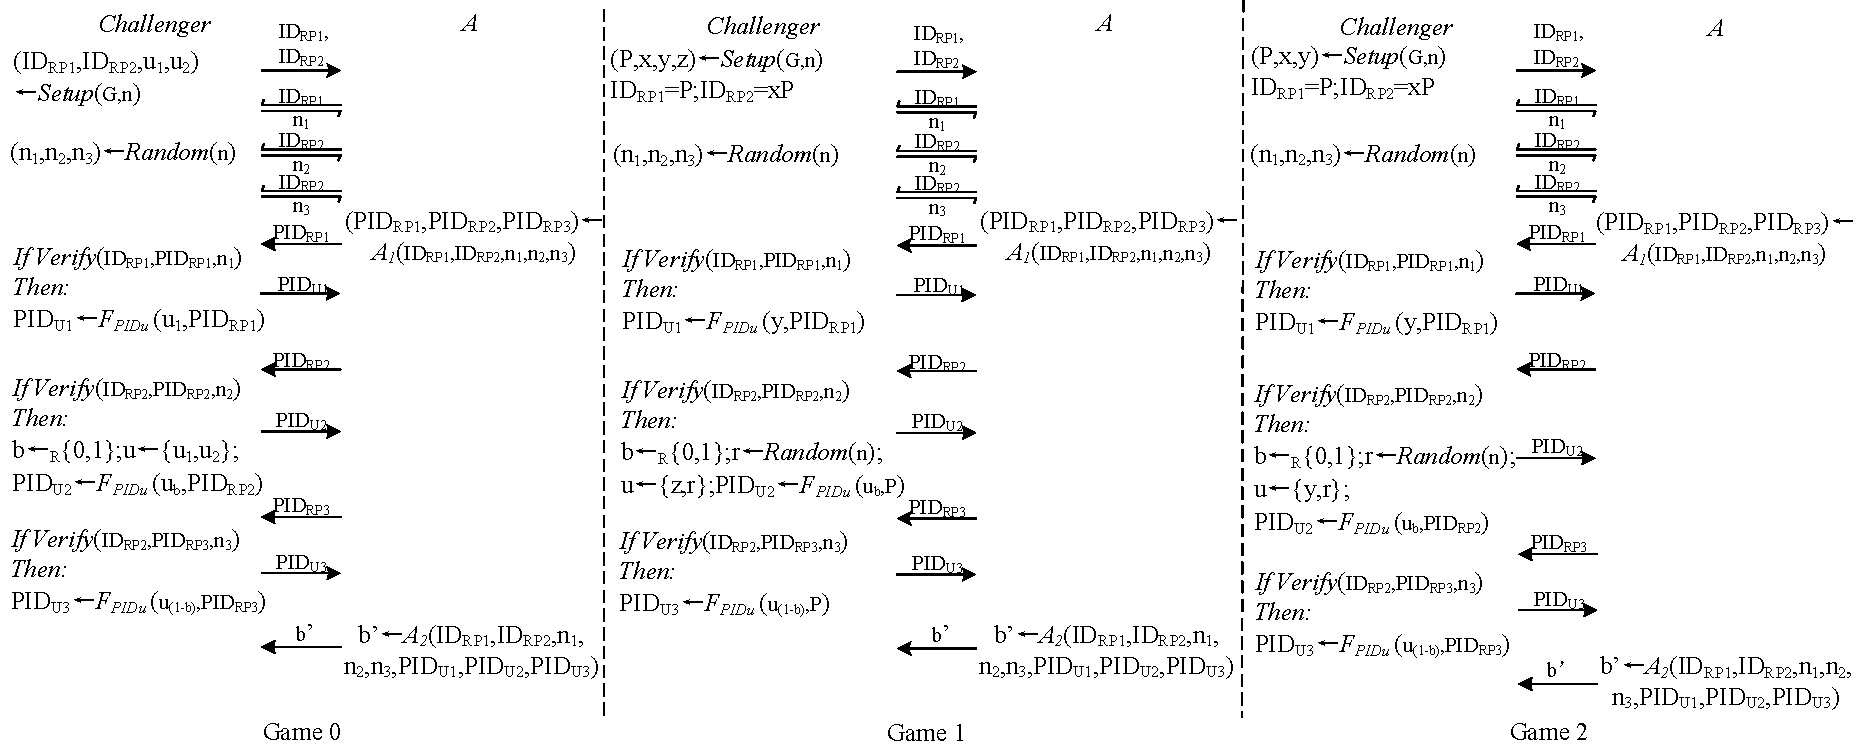
\includegraphics[width=\textwidth, height=0.35\textheight]{fig/game.pdf}
\captionof{figure}{Interactions between the challenger and the adversary in three Games.}
\label{fig:game}
\vspace{-5mm}
\end{strip}


\begin{comment}

Next, we model the guessing Game to depict the interactions between the challenger and the adversary. First, we describe the challenger's actions in the Game as follows.
\begin{itemize}
\vspace{-\topsep}
\item[-] {\em Initialization:} In initialization, the challenger generates $ID_{RP}$s and $ID_U$s for multiple RPs and users using the initialization algorithm $Setup(G,n)$, where $G$ and $n$ are defined in table~\ref{tbl:notations}.
\vspace{-\topsep}
\item[-] {\em Random number generation:} When the challenger receives the $ID_{RP}$s from the adversary, it generates a random $N_U \in \mathbb{Z}_n$ for each $ID_{RP}$ using the algorithm $Random(n)$. %$N_U$ will be used to generate the corresponding $PID_{RP}$.
\vspace{-\topsep}
\item[-] {\em $PID_U$ generation:} When the challenger receives an $PID_{RP}$, it first verifies if the $PID_{RP}$ is generated for $ID_{RP}$ with the corresponding $N_U$, using the algorithm $Verify(ID_{RP},PID_{RP},N_U)$. Then, it generates the $PID_U$ with the algorithm $F_{PID_U}(ID_U,PID_{RP})$ and sends it to the adversary.
%\vspace{-\topsep}
\end{itemize}

To prove the privacy of UPPRESSO against RP-based identity linkage, we define three Games, as shown in figure~\ref{fig:game}. First, based on the above description, we model the $ID_U$-guessing game following the UPPRESSO design as $\mathtt{Game 0}$ : (1) First, the adversary receives two $ID_{RP}$s (i.e., $ID_{RP1}$ and $ID_{RP2}$) and three $N_U$s (i.e., $n_1$, $n_2$, and $n_3$). It then generates three $PID_{RP}$s accordingly. From the challenger's view, three $PID_{RP}$s are related to three $N_U$s, respectively. (2) Then, the challenger generates $PID_U$s for different $PID_{RP}$s, using two $ID_U$s (i.e., $u_1$ and $u_2$). %generated in the initialization phase.
In particular, the challenger generates $PID_{U1}$ from $ID_{U1}$ directly, and selects a random number $b \in \{0, 1\}$ to generate $PID_{U2}=ID_{Ub} \cdot PID_{RP2}$, and $PID_{U3}=ID_{U(1-b)} \cdot PID_{RP3}$. (3) Finally, the adversary sends its guess $b'$ to the challenger. If $b'=b$, the adversary wins the game.

We define the event [$b'=b$] in $\mathtt{Game 0}$ as $\Gamma$. If the adversary has no advantage in guessing $b$ correctly, which indicates the $PID_U$s are generated from the same $ID_U$, the probability $Pr[\Gamma]$ should be 1/2. Therefore, we conclude that in $\mathtt{Game 0}$, UPPRESSO is secure against RP-based identity linkage if and only if $Pr[\Gamma]=1/2$.


Next, we build the ideal model of the guessing game, denoted as $\mathtt{Game 1}$. In this model, the probability that the adversary correctly guessing $b$ is 1/2. This time, the challenger randomly selects $z$ and $r$ and uses them to generate $PID_{U2}$ and $PID_{U3}$, respectively. Since the adversary does not know $z$ and $r$, he does not know $b$ neither. Similarly, we define the event [$b'=b$] in $\mathtt{Game 1}$ as $\Gamma_1$, and $Pr[\Gamma_1]$ should be 1/2.

According to the DDH assumption, we need to prove that $|Pr[\Gamma_1]-Pr[\Gamma]|=\sigma(n)$, where $\sigma(n)$ is negligible. So, we build another model of Game, denoted as $\mathtt{Game 2}$, by setting the values of the parameters defined in $\mathtt{Game 0}$ to be: $ID_{RP2}=xID_{RP1}$, $u_1=y$ and $u_2=r$, where $r$ is a random number. Again, we define the event [$b'=b$] in  $\mathtt{Game 2}$ as $\Gamma_2$, and $Pr[\Gamma_2]=Pr[\Gamma]$ should be true.

After defining the three games, we prove that $|Pr[\Gamma_1]-Pr[\Gamma_2]|=\sigma(n)$ as follows. In each game, the adversary uses the algorithm $A_2$ to derive $b'$ from the collected data, i.e., $\{ID_{RP1},ID_{RP2},n_1,n_2,n_3,PID_{U1},PID_{U2},PID_{U3}\}$. Now, let us replace the parameters in $\mathtt{Game 1}$ and $\mathtt{Game 2}$ with the exact values:
\vspace{-\topsep}
\begin{equation*}
\begin{aligned}
    b'_{game1} \gets A_2(P,xP,n_1,n_2,n_3,yn_1P,zP,rP) \\
    b'_{game2}\gets A_2(P,xP,n_1,n_2,n_3,yn_1P,xyn_2P,rn_3P) \\
    or \; b'_{game2}\gets A_2(P,xP,n_1,n_2,n_3,yn_1P,rn_2P,xyn_3P)
\end{aligned}
\end{equation*}
\vspace{-\topsep}

Since $n_1$, $n_2$, $n_3$ are randomly chosen by the challenger, which are not related to $ID_U$, the adversary can easily remove them and obtain $b'_{game1}\gets A_2(P,xP,yP,zP,rP)$ in $\mathtt{Game 1}$ and $b'_{game2}\gets A_2(P,xP,yP,xyP,xrP)$ in $\mathtt{Game 2}$.

As $r$ is randomly chosen and unknown to the adversary, $rP$ and $xrP$ are also random points. We can re-write $b'_{game1}$ and $b'_{game2}$ as $b'_{game1}\gets A_2(P,xP,yP,zP,r_1P)$ and $b'_{game2}\gets A_2(P,xP,yP,xyP,r_2P)$, which means there is no non-negligible difference between the success probability in $\mathtt{Game 1}$ and $\mathtt{Game 2}$, according to the DDH assumption. Otherwise, we should be able to build a PPT distinguishing algorithm that breaks DDH assumption about the adversary.

Such distinguishing algorithm $D$ is shown in figure~\ref{fig:dalgorithm}.
The inputs of the algorithm is $\{P,X,Y,Z\}$. To the adversary, it is $\mathtt{Game 1}$ if the input is in the form $\{P,xP,yP,zP\}_{x,y,z \in \mathbb{Z}_n}$, and it is $\mathtt{Game 1}$ if the input is $\{P,xP,yP,xyP\}_{x,y \in \mathbb{Z}_n}$. As a result,
\vspace{-\topsep}
\begin{multline*}
   \ \ \ \ \ \ \ \ \ \ \ \ \ \ \ \ \  Pr[D(P,xP,yP,zP)=1]=Pr[{\Gamma_1}]\\
   Pr[D(P,xP,yP,xyP)=1]=Pr[{\Gamma_2}]\ \ \ \ \ \ \ \ \ \ \ \ \ \ \ \ \ \
\end{multline*}

\vspace{-\topsep}
Therefore, $|Pr[\Gamma_1]-Pr[\Gamma_2]|=\sigma(n)$, where $\sigma(n)$ is negligible, and $n$ is the security parameter. It means the adversary has no advantage in guessing $b$ in $\mathtt{Game 0}$. Therefore, he cannot distinguish if two $PID_U$s at two different RPs belong to the same user or not. This proves that UPPRESSO is resistant to RP-based identity linkage attacks.

\end{comment}


\begin{comment}
\begin{figure}[t]
  \centering
  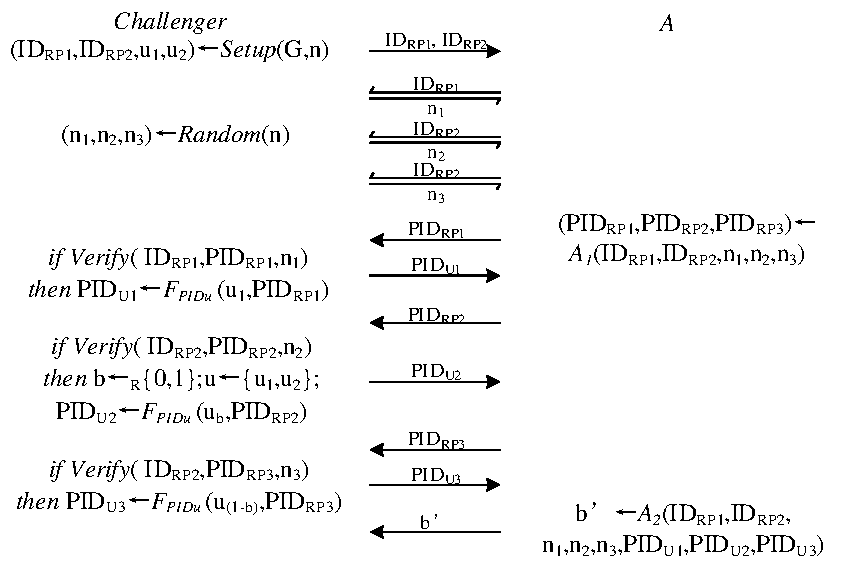
\includegraphics[width=1\linewidth]{fig/game0.pdf}
  \vspace{-5mm}
  \caption{Game 0.}
  \label{fig:game0}
  \vspace{-5mm}
\end{figure}


\begin{figure}[t]
  \centering
  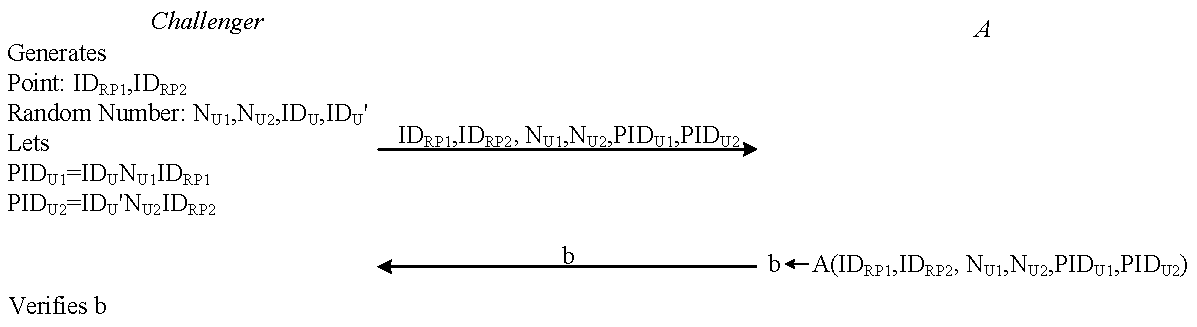
\includegraphics[width=1\linewidth]{fig/game1.pdf}
  \vspace{-5mm}
  \caption{Game 1.}
  \label{fig:game1}
    \vspace{-5mm}
\end{figure}

\begin{figure}[t]
  \centering
  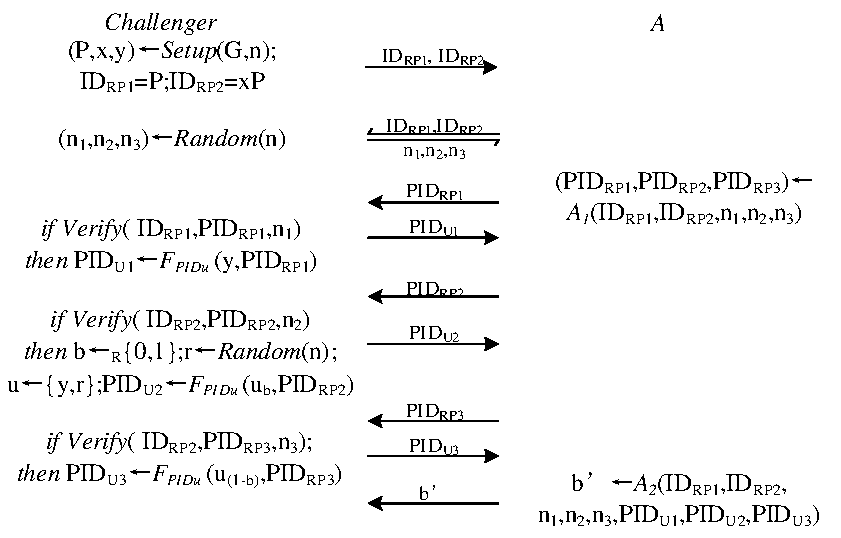
\includegraphics[width=1\linewidth]{fig/game2.pdf}
  \vspace{-5mm}
  \caption{Game 2.}
  \label{fig:game2}
  \vspace{-5mm}
\end{figure}

\end{comment}

%\end{appendices}
